\section{Parallel KNN}
% See ESLII page 33
% See Dirk page
The $k^{th}$ Nearest-Neighbor (k-NN) methods uses observations from a training set $T$ to find its closest neighbours in feature space to a given an unknown sample $\bm{x}$ a prediction value $\overline{y}$ \cite{HastieTrevor2009EoSL}. The prediction for the k-NN classifier is usually calculated as an average or consensus vote, that is
\[
    \overline{y} \left( \bm{x} \right) = \sum_{\bm{x}_{i} \in N_{k} (\bm{x})} y_{i}
\]
The notion of 'closest' implies the use of some sort of metric. More often than not, feature vectors belong to to some subset $\mathbb{R}^{n}$, allowing us to apply commonly used metrics to define distance between vectors in our feature space. For our purposes, we shall use the Euclidean norm as a measurement of determining how close two feature values are to each other. The Euclidean norm is simply defined as
\[
    d \left( \bm{x}, \bm{y} \right) = \left( \sum_{i=1}^{n} \left( x_{i} - y_{i} \right)^{2} \right)^{\frac{1}{2}}.
\]
Other metrics such as Manhatten norm or hamming distance for discrete feature spaces \cite{HastieTrevor2009EoSL}. When a unknown sample $\bm{x}$ is to be classified, a k-NN classifier computes the distance between $\bm{x}$ and the other points within the training set $T$. The training data is then sorted by distance and the $k^{th}$ closests training samples are then used to predict $\bm{x}$. A simple K-NN algorithm is presented in algorithm \ref{alg:serial-k-NN}.
\begin{algorithm}[ht!!!]
\caption{Serial k-NN}
\label{alg:serial-k-NN}
\SetAlgoLined
    \SetKwInOut{Input}{input}\SetKwInOut{Output}{output}
    
    \Input{Training data $T$, an unlabelled sample $\bm{x}$ and a value $k$}
    \Output{Predicted class $\overline{y} \left( \bm{x} \right)$}
    \BlankLine
    Computes distance $d \left( \bm{x}, \bm{x}_{t_i} \right)$ for each $\bm{x}_{t_i} \in T$\;
    $N_{k} (\bm{x}) \gets$ the $k^{th}$ closest $\bm{x}_{t_i}$ determined by $d \left( \bm{x}, \bm{x}_{t_i} \right)$\;
    $\overline{y} \left( \bm{x} \right) \gets \sum_{\bm{x}_{i} \in N_{k} (\bm{x})} y_{i}$\;
    \KwResult{$\overline{y} \left( \bm{x} \right)$}
    \BlankLine
\end{algorithm}
While this method is simple, computing the distance between $\bm{x}$ and each $\bm{x}_{t_i} \in T$ can incur a large time overhead, especially for large training sets. In order to parallize this algorithm, one important observation is that computing the distances $d \left( \bm{x}, \bm{x}_{t_i} \right)$ and $d \left( \bm{x}, \bm{x}_{t_j} \right)$ where $\bm{x}_{t_i}, \bm{x}_{t_j} \in T$ and $i \neq j$ allowing us to carry out these computations on separate processes. Liang et al. (2010) takes advantage of this independence by splitting up the training examples into $p$ partitions and send these partitions to slave processes to compute the distances between feature vectors in our training example and a unknown sample $\bm{x}$. The $k^{th}$ closet training examples are found within individual slaves and are collected within the master process. Combining the $k^{th}$ closet acquired by each process locally, the master process then sorts the reduced list of training vectors to find the global $k^{th}$ closet training examples \cite{ShenshenLiang2010Daeo}. Pseudo code for parallel KNN is shown in \ref{alg:parallel-k-NN}.
\begin{algorithm}[h!!!]
\caption{Parallel k-NN}
\label{alg:parallel-k-NN}
\SetAlgoLined
    \SetKwInOut{Input}{input}\SetKwInOut{Output}{output}
    \Input{Training data $T$, an unlabelled sample $\bm{x}$, a value $k$ and the number of processes to perform the algorithm $p$}
    \Output{Predicted class $\overline{y} \left( \bm{x} \right)$}
    \BlankLine
    $\left\lbrace T_{1} , T_{2}, \ldots , T_{p} \right\rbrace \gets$ an equal partition of $T$\;
    \For{$T_{i} \in \left\lbrace T_{1} , T_{2}, \ldots , T_{p} \right\rbrace$ {\bf concurrently}}{
        $N_{k_i} (\bm{x}) \gets$ the $k^{th}$ nearest neighbors from $T_{i}$\;
    }
    $N_{k} (\bm{x}) \gets$ the $k^{th}$ closest neighbors from $N_{k_1} (\bm{x}), N_{k_2} (\bm{x}), \ldots N_{k_p} (\bm{x})$\;
    $\overline{y} \left( \bm{x} \right) \gets \sum_{\bm{x}_{i} \in N_{k} (\bm{x})} y_{i}$\;
    \KwResult{$\overline{y} \left( \bm{x} \right)$}
    \BlankLine
\end{algorithm}

This algorithm is shown pictorially below\\
\renewcommand{\labelenumi}{\textbf{Step \arabic{enumi})}}
\begin{enumerate}
    \item Partition the data and send partitions to processes \(P_{1}, P_{2}, P_{3}, P_{4}\)
    \begin{figure}[H]
        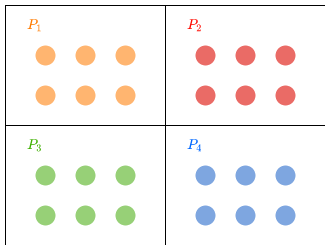
\includegraphics[scale=0.8]{img/STAT4402_tut_KNN_1_no_cap.png}
        \centering
    \end{figure}
    
    \item Determine the closest samples within each process
    \begin{figure}[H]
        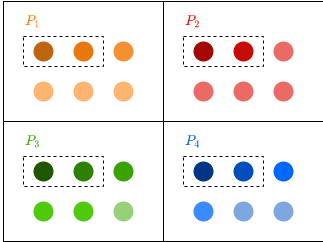
\includegraphics[scale=0.8]{img/STAT4402_tut_KNN_2_no_cap.png}
        \centering
    \end{figure}
    
    \item Collect the \(k^{th}\) closest samples and order them in the master node get the global
\(k^{th}\) closest samples
    \begin{figure}[H]
        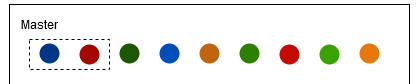
\includegraphics[scale=0.7]{img/STAT4402_tut_KNN_3_no_cap.png}
        \centering
    \end{figure}
\end{enumerate}